\chapter{बीज से पौधे तक}\label{ch:g2:from-seed-to-plant}

सेम की सूखी फली हिलाओ और छोटे-छोटे सख़्त \omterm{def:g2:from-seed-to-plant:seed}{बीज} खड़खड़ाकर बाहर गिरते हैं
--- सूखे, फीके, देखने में रोड़ी जितने ही निर्जीव। फिर भी उनमें से एक
को मिट्टी में बोकर पानी दो, और कुछ ही दिनों में ज़मीन के नीचे कुछ
असाधारण घटता है। भीतर एक पूरा \omterm{def:g1:plants-around-us:plant}{पौधा} तह किया हुआ पड़ा था, अपने संकेत के
इंतज़ार में।

\section{बीज क्या है}

\begin{definition}[बीज]\label{def:g2:from-seed-to-plant:seed}
\emph{बीज}\index{बीज} किसी नए \omterm{def:g1:plants-around-us:plant}{पौधे} की शुरुआत है, जिसे जनक \omterm{def:g1:plants-around-us:plant}{पौधे} ने
बनाया है। अपने रक्षक छिलके के भीतर बीज लिए रहता है:
\begin{itemize}
  \item एक नन्हा \omterm{def:g1:plants-around-us:plant}{पौधा} जो शुरू हो चुका है --- \omterm{def:g1:plants-around-us:plant}{पौधे} का
        \emph{भ्रूण}\index{भ्रूण (बीज का)}, जिसमें एक \omterm{def:g1:plants-around-us:parts}{जड़} और एक
        \omterm{prop:g2:from-seed-to-plant:cycle}{अंकुर} की शुरुआत होती है;
  \item भोजन का एक भंडार, जो उसे तब तक खिलाए जब तक वह ख़ुद न खा सके।
\end{itemize}
\end{definition}

\begin{example}[भिगोया सेम खोलना]\label{ex:g2:from-seed-to-plant:open}
किसी बड़े सफ़ेद सेम को रात भर भिगो दो, और उसका छिलका आसानी से उतर आता
है। सेम दो मोटे टुकड़ों में खुल जाता है --- वही भोजन का भंडार --- और
वहीं, एक किनारे से सटा हुआ, चावल के दाने जितना छोटा एक पीला-सा \omterm{def:g1:plants-around-us:plant}{पौधा}
पड़ा होता है, \omterm{def:g1:plants-around-us:parts}{जड़} की नोक और तह की हुई पहली \omterm{def:g1:plants-around-us:parts}{पत्तियों} के साथ। नया \omterm{def:g1:plants-around-us:plant}{पौधा}
शुरू से ही वहाँ था।
\end{example}

\begin{omfigure}
\begin{tikzpicture}
  \node[anchor=south west, inner sep=0] (img) at (0,0)
    {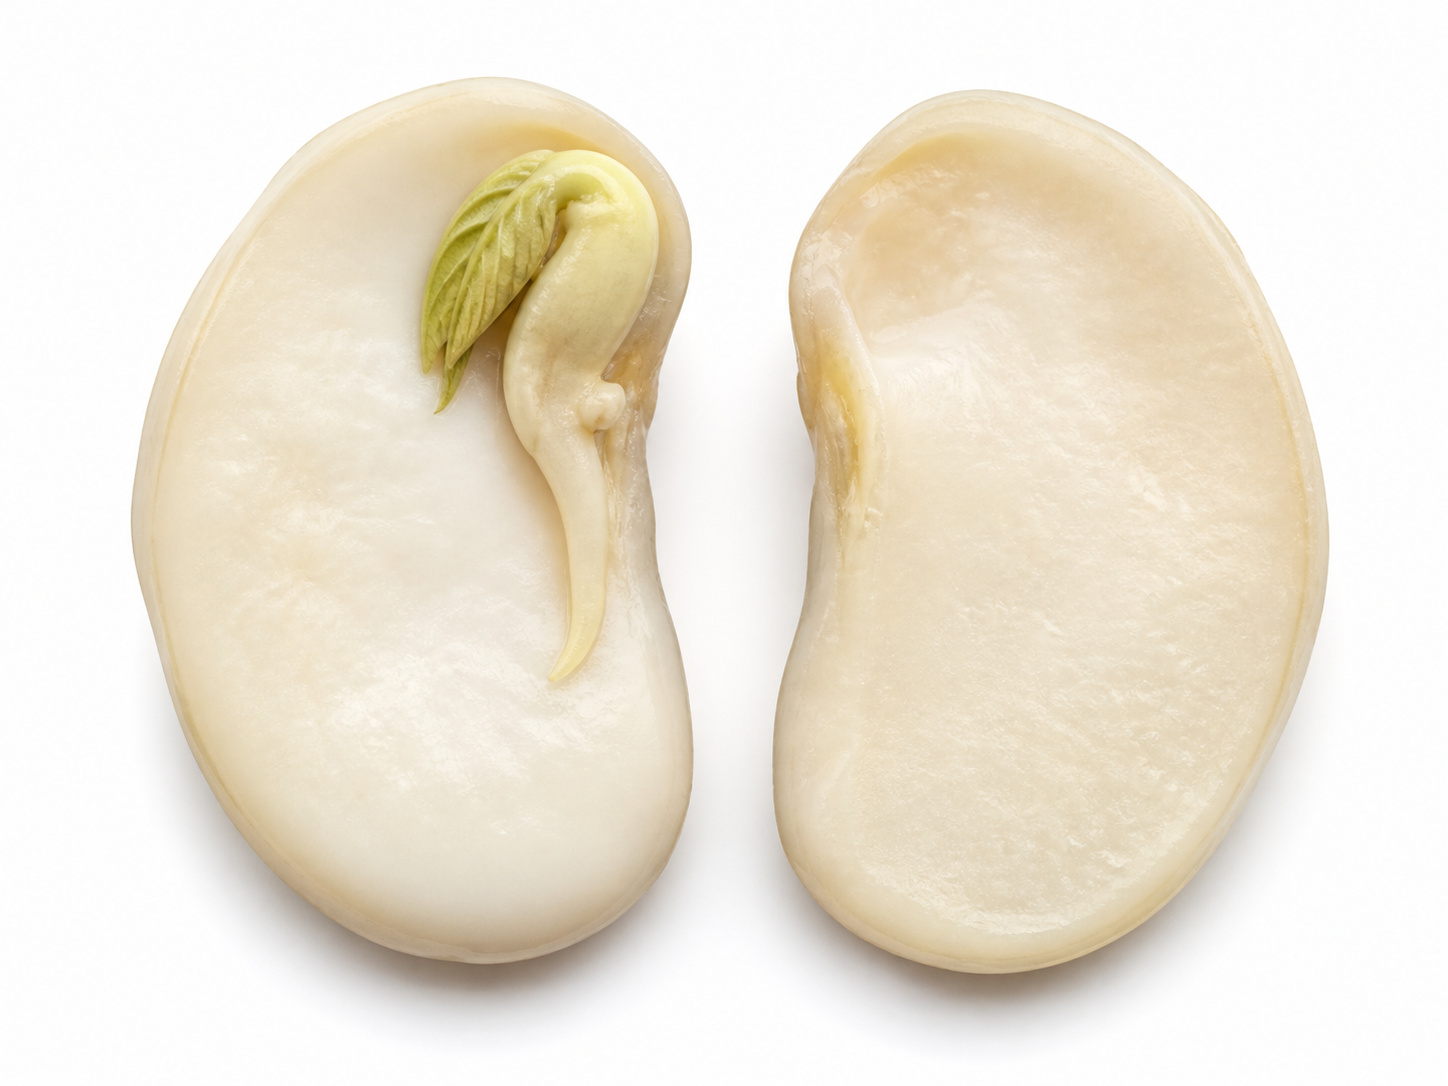
\includegraphics[width=0.62\linewidth]{images/book1/ai/fig-bean-open.png}};
  \begin{scope}[x={(img.south east)}, y={(img.north west)},
      every node/.style={font=\small}]
    \draw[omDef, thick] (0.35,0.79) -- (0.26,0.94)
      node[above] {तह की हुई पहली पत्तियाँ};
    \draw[omDef, thick] (0.40,0.38) -- (0.28,-0.04)
      node[below] {जड़ की नोक};
    \draw[omDef, thick] (0.78,0.35) -- (0.80,-0.04)
      node[below, align=center] {दो मोटे टुकड़े:\\ भोजन का भंडार};
  \end{scope}
\end{tikzpicture}

{\small भिगोकर खोले गए सेम के भीतर: एक नन्हा \omterm{def:g1:plants-around-us:plant}{पौधा} --- \omterm{def:g1:plants-around-us:parts}{जड़} की नोक और
तह की हुई पहली \omterm{def:g1:plants-around-us:parts}{पत्तियाँ} --- अपने भोजन-भंडार से सटा हुआ।}
\end{omfigure}

\begin{remark}[बीज हमारी रसोई से गुज़रते हैं]\label{rem:g2:from-seed-to-plant:kitchen}
सेम, मटर, मसूर, चावल, सूरजमुखी के \omterm{def:g2:from-seed-to-plant:seed}{बीज}, सेब के दाने और आड़ू की गुठली:
रसोई \omterm{def:g2:from-seed-to-plant:seed}{बीजों} से भरी है। कुछ बहुत छोटे हैं, जैसे ख़सख़स के \omterm{def:g2:from-seed-to-plant:seed}{बीज}; नारियल
उनमें से एक विशाल \omterm{def:g2:from-seed-to-plant:seed}{बीज} है। मौक़ा मिले तो इनमें से हर एक \omterm{def:g1:plants-around-us:plant}{पौधा} बनने की
कोशिश करेगा।
\end{remark}

\section{अंकुरण}

\begin{definition}[अंकुरण]\label{def:g2:from-seed-to-plant:germination}
\emph{अंकुरण}\index{अंकुरण} वह घड़ी है जब \omterm{def:g2:from-seed-to-plant:seed}{बीज} जागता है और बढ़ना शुरू
करता है: वह पानी सोखकर फूलता है, उसका छिलका फटता है, सबसे पहले नन्ही
\omterm{def:g1:plants-around-us:parts}{जड़} बाहर आकर नीचे की ओर गोता लगाती है, फिर \omterm{prop:g2:from-seed-to-plant:cycle}{अंकुर} उठता है और पहली हरी
\omterm{def:g1:plants-around-us:parts}{पत्तियाँ} प्रकाश की ओर ले जाता है। हम कहते हैं कि \omterm{def:g2:from-seed-to-plant:seed}{बीज}
\emph{अंकुरित होता है}\index{अंकुरित होना}।
\end{definition}

\begin{proposition}[अंकुरण के लिए बीज को क्या चाहिए]\label{prop:g2:from-seed-to-plant:needs}
\omterm{def:g2:from-seed-to-plant:germination}{अंकुरित होने} के लिए \omterm{def:g2:from-seed-to-plant:seed}{बीज} को \emph{पानी} और \emph{गरमाहट} चाहिए। उसे
अभी प्रकाश नहीं चाहिए: शुरू में भोजन-भंडार ही \omterm{prop:g2:from-seed-to-plant:cycle}{अंकुर} को खिलाता है,
मिट्टी के नीचे अँधेरे में भी। पानी के बिना, या ठंड में, अच्छा \omterm{def:g2:from-seed-to-plant:seed}{बीज} बस
इंतज़ार करता रहता है।
\end{proposition}
\admitted

\begin{example}[बुआई वसंत का इंतज़ार क्यों करती है]\label{ex:g2:from-seed-to-plant:spring}
माली सेम वसंत में बोते हैं, सर्दियों में नहीं: ठंडी मिट्टी में \omterm{def:g2:from-seed-to-plant:seed}{बीज}
\omterm{def:g2:from-seed-to-plant:germination}{अंकुरित होने} के बजाय इंतज़ार करता --- या सड़ जाता। गरम दिन और सींची
हुई मिट्टी ठीक \cref{prop:g2:from-seed-to-plant:needs} के दो संकेत
हैं।
\end{example}

\begin{method}[बीज बोकर उसका अंकुरण देखना]\label{met:g2:from-seed-to-plant:sow}
\begin{enumerate}
  \item काँच के मरतबान को नम रुई या काग़ज़ से अस्तर कर दो;
  \item काँच और रुई के बीच एक सेम सरका दो, ताकि वह दिखता रहे;
  \item मरतबान को गरम कमरे में रखो और रुई नम बनाए रखो;
  \item रोज़ देखो और जो दिखे उसे लिखो: फूलना, छिलके का फटना, \omterm{def:g1:plants-around-us:parts}{जड़} का
        नीचे जाना, \omterm{prop:g2:from-seed-to-plant:cycle}{अंकुर} का ऊपर आना।
\end{enumerate}
काँच वह सब दिखा देता है जो आम तौर पर मिट्टी के नीचे होता है।
\end{method}

\begin{omfigure}
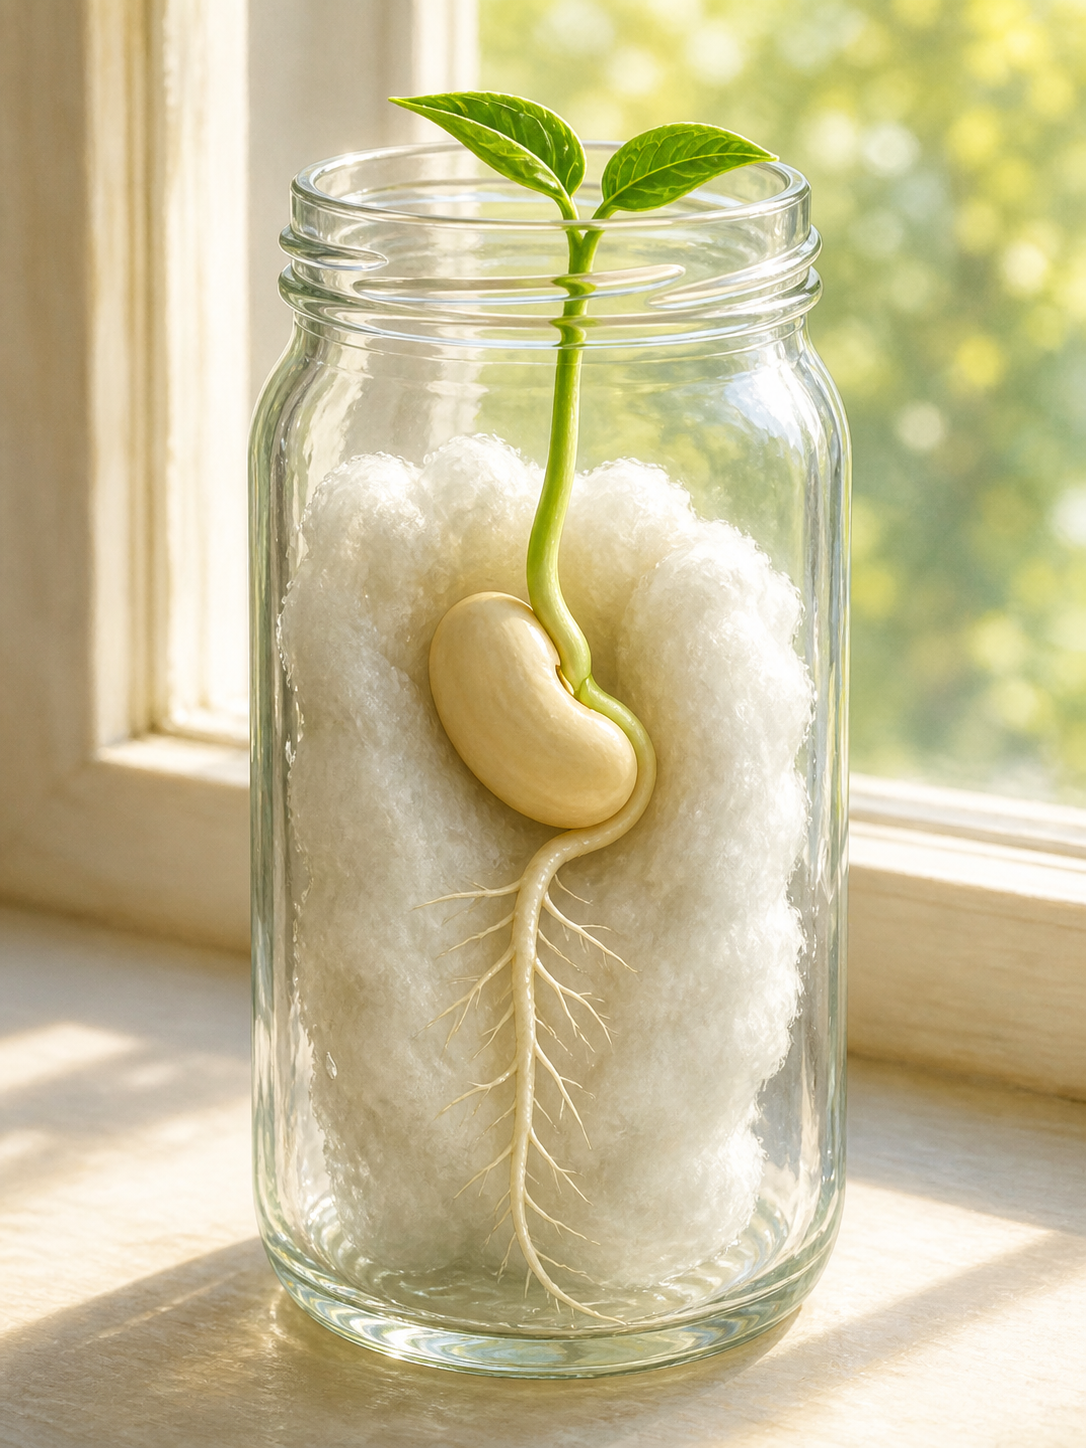
\includegraphics[width=0.44\linewidth]{images/book1/ai/g2-seed-bean-jar.png}

{\small \omterm{def:g2:from-seed-to-plant:germination}{अंकुरण} के बीचोंबीच मरतबान वाला प्रयोग: \omterm{def:g1:plants-around-us:parts}{जड़} नीचे, \omterm{prop:g2:from-seed-to-plant:cycle}{अंकुर} ऊपर,
और बीच में ख़ाली होता \omterm{def:g2:from-seed-to-plant:seed}{बीज}।}
\end{omfigure}

\begin{remark}[जड़ नीचे, अंकुर ऊपर --- हमेशा]\label{rem:g2:from-seed-to-plant:updown}
मरतबान में सेम चाहे जैसे भी पड़ा हो --- बग़ल के बल, उलटा --- \omterm{def:g1:plants-around-us:parts}{जड़} हमेशा
नीचे की ओर मुड़ती है और \omterm{prop:g2:from-seed-to-plant:cycle}{अंकुर} हमेशा ऊपर की ओर। \omterm{prop:g2:from-seed-to-plant:cycle}{अंकुर} देख नहीं सकता,
फिर भी वह जानता है कि ऊपर किधर है। \omterm{def:g1:plants-around-us:plant}{पौधे} जितना दिखाते हैं, उससे ज़्यादा
भाँपते हैं।
\end{remark}

\section{अंकुर से लेकर बीज वाले पौधे तक}

\begin{proposition}[पौधे का जीवन चक्र]\label{prop:g2:from-seed-to-plant:cycle}
\emph{अंकुर}\index{अंकुर} बढ़कर \omterm{def:g1:plants-around-us:parts}{जड़ों}, \omterm{def:g1:plants-around-us:parts}{डंठल} और \omterm{def:g1:plants-around-us:parts}{पत्तियों} वाला \omterm{def:g1:plants-around-us:plant}{पौधा} बन
जाता है; \omterm{def:g1:plants-around-us:plant}{पौधे} में \omterm{def:g1:plants-around-us:parts}{फूल} आते हैं; \omterm{def:g1:plants-around-us:parts}{फूल} नए \emph{\omterm{def:g2:from-seed-to-plant:seed}{बीज}} बनाते हैं; और चक्र
फिर से शुरू हो सकता है। सेम का एक ही \omterm{def:g1:plants-around-us:plant}{पौधा} एक गर्मी में दर्जनों नए सेम
बना सकता है।
\end{proposition}
\admitted

\begin{example}[एक सेम, एक गर्मी]\label{ex:g2:from-seed-to-plant:summer}
मई में बोया गया सेम हफ़्ते भर में अंकुरित हो जाता है; जून तक वह अपने
खंभे पर चढ़ता पत्तेदार \omterm{def:g1:plants-around-us:plant}{पौधा} है; जुलाई में सफ़ेद \omterm{def:g1:plants-around-us:parts}{फूल} आते हैं, फिर हरी
फलियाँ; अगस्त में फलियाँ भारी होकर लटकती हैं, हर एक में नए सेमों की
एक क़तार --- अगले साल के \omterm{def:g2:from-seed-to-plant:seed}{बीज}, इस साल के \omterm{def:g1:plants-around-us:plant}{पौधे} के बनाए हुए।
\end{example}

\section{अभ्यास}

\begin{exercise}[$\star$]\label{exo:g2:from-seed-to-plant:1}
\omterm{def:g2:from-seed-to-plant:seed}{बीज} के छिलके के भीतर कौन-सी दो चीज़ें होती हैं?
\end{exercise}

\begin{exercise}[$\star$]\label{exo:g2:from-seed-to-plant:2}
\emph{\omterm{def:g2:from-seed-to-plant:germination}{अंकुरित होना}} का क्या अर्थ है? \omterm{def:g2:from-seed-to-plant:seed}{बीज} से सबसे पहले क्या बाहर आता
है: \omterm{def:g1:plants-around-us:parts}{जड़}, या \omterm{prop:g2:from-seed-to-plant:cycle}{अंकुर}?
\end{exercise}

\begin{exercise}[$\star$]\label{exo:g2:from-seed-to-plant:3}
\omterm{def:g2:from-seed-to-plant:germination}{अंकुरित होने} के लिए \omterm{def:g2:from-seed-to-plant:seed}{बीज} को ज़रूरी दो चीज़ें बताओ। बड़े \omterm{def:g1:plants-around-us:plant}{पौधों} की कौन-सी
मशहूर ज़रूरत इस सूची में \emph{नहीं} है?
\end{exercise}

\begin{exercise}[$\star$]\label{exo:g2:from-seed-to-plant:4}
मिट्टी में दबा \omterm{prop:g2:from-seed-to-plant:cycle}{अंकुर} प्रकाश तक पहुँचने से पहले अँधेरे में कैसे बढ़
सकता है? शुरू में उसका भोजन कहाँ से आता है?
\end{exercise}

\begin{exercise}[$\star$]\label{exo:g2:from-seed-to-plant:5}
रसोई में मिल सकने वाले चार \omterm{def:g2:from-seed-to-plant:seed}{बीजों} के नाम बताओ।
\end{exercise}

\begin{exercise}[$\star$]\label{exo:g2:from-seed-to-plant:6}
माली सर्दियों के बजाय वसंत में क्यों बोते हैं?
\end{exercise}

\begin{exercise}[$\star$]\label{exo:g2:from-seed-to-plant:7}
क्रम में लगाओ: नए सेमों वाली फली --- \omterm{def:g2:from-seed-to-plant:seed}{बीज} --- \omterm{def:g1:plants-around-us:parts}{फूल} वाला \omterm{def:g1:plants-around-us:plant}{पौधा} ---
\omterm{prop:g2:from-seed-to-plant:cycle}{अंकुर} --- पत्तेदार \omterm{def:g1:plants-around-us:plant}{पौधा}।
\end{exercise}

\begin{exercise}[$\star$]\label{exo:g2:from-seed-to-plant:8}
करके देखो: \cref{met:g2:from-seed-to-plant:sow} वाला काँच का मरतबान
दो सेमों के साथ लगाओ --- एक बग़ल के बल, एक उलटा। \omterm{def:g2:from-seed-to-plant:germination}{अंकुरण} के बाद उनकी
\omterm{def:g1:plants-around-us:parts}{जड़ों} और \omterm{prop:g2:from-seed-to-plant:cycle}{अंकुरों} की तुलना करो।
\cref{rem:g2:from-seed-to-plant:updown} क्या भविष्यवाणी करता है?
\end{exercise}

\begin{exercise}[$\star\star$]\label{exo:g2:from-seed-to-plant:9}
नीना सेम के \omterm{def:g2:from-seed-to-plant:seed}{बीजों} का पैकेट पूरे एक साल सूखी दराज़ में रखती है, और
आख़िर में बोने पर वे फिर भी अंकुरित हो जाते हैं। दराज़ में वे न बढ़े
और न मरे, ऐसा क्यों? \cref{prop:g2:from-seed-to-plant:needs} का
इस्तेमाल करो।
\end{exercise}

\begin{exercise}[$\star\star$]\label{exo:g2:from-seed-to-plant:10}
\cref{ch:g2:animals-grow-up} का चूज़ा अपने \omterm{def:g2:animals-grow-up:born}{अंडे} के भीतर बढ़ता है,
जिसे ज़र्दी खिलाती है। सेम के भीतर ज़र्दी की भूमिका कौन निभाता है?
\omterm{def:g2:animals-grow-up:born}{अंडे} और \omterm{def:g2:from-seed-to-plant:seed}{बीज} में क्या बात एक जैसी है?
\end{exercise}
